\section{Results}
Selected preprocessing / serving / mapping approaches
Survey results
The map application

\subsection{Data preprocessing}

\subsection{Application design}

See table \ref{tab:map library comparison} for comparison of mapping libraries.


% TODO Describe why these libraries were selected
% Baseline: FOSS, Actively maintained, usable with UI framework
% Discarded: Openlayers (no integration to react) Mapbox (closed source)
% Integration with react -> developer experience & maintainability

\begin{table}[H]
	\caption{Comparison of mapping libraries}
	\label{tab:map library comparison}
	\centering
	\begin{tabular}{ | L{0.1\textwidth} | L{0.25\textwidth} | L{0.25\textwidth} | L{0.25\textwidth} | }
		\hline
		Library
		& Quality of visualization
		& Rendering performance
		& Integration with React
		\\ 
		\hline
		\hline
		Deck.gl
		& Inconsistent rendering of complex polygons, vector tiles supported
		& GPU accelerated (WebGL), most performant of the tested libraries
		& Designed from ground up to work with React
		\\
		\hline
		Leaflet
		& Correct rendering of polygons, Vector tiles possible through plugins
		& No GPU acceleration, least performant of the tested libraries
		& Integration possible with a 3rd party wrapper
		\\
		\hline
		Maplibre
		& Correct rendering of polygons with very rare inconsistencies, vector tiles supported
		& GPU accelerated (WebGL), slightly less performant than deck.gl
		& Integration possible with a 3rd party wrapper
		\\
		\hline
	\end{tabular}
\end{table}


\subsection{Map usage}

See \ref{fig:q 1 and 2} for answers to questions 1 \ref{fig:q 1} and 2 \ref{fig:q 2}.

\begin{figure}[H]
	\centering
	\begin{subfigure}[b]{0.5\textwidth}
		\centering
		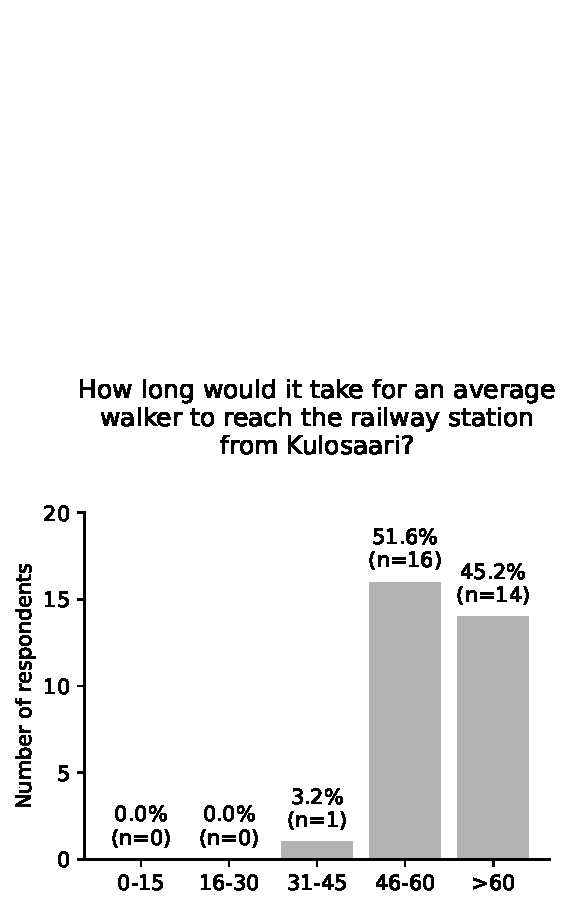
\includegraphics[width=\textwidth]{visual/figures/survey/0.pdf}
		\caption{Question 1}
		\label{fig:q 1}
	\end{subfigure}%
	\hfill
	\begin{subfigure}[b]{0.5\textwidth}
		\centering
		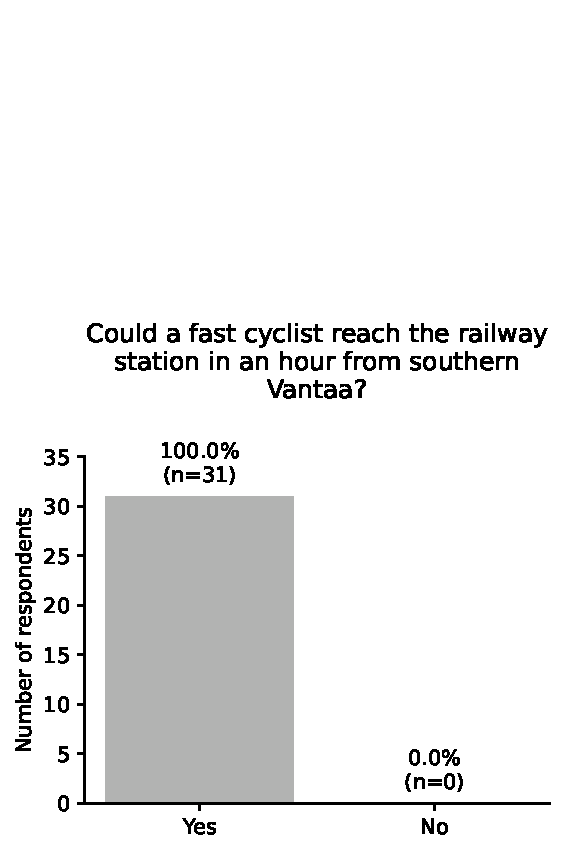
\includegraphics[width=\textwidth]{visual/figures/survey/1.pdf}
		\caption{Question 2}
		\label{fig:q 2}
	\end{subfigure}%
	\caption{Questions 1 and 2}
	\label{fig:q 1 and 2}
\end{figure}

\begin{figure}[H]
	\centering
	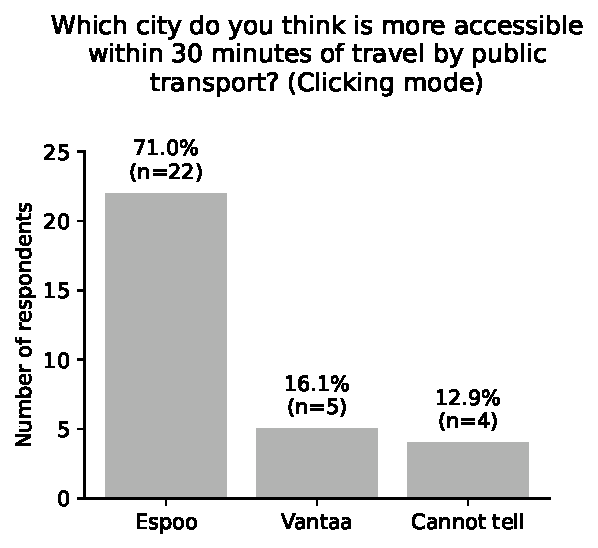
\includegraphics[width=0.5\textwidth]{visual/figures/survey/2.pdf}
	\caption{Question 3}
	\label{fig:q 3}
\end{figure}

\begin{figure}[H]
	\centering
	\begin{subfigure}[b]{0.5\textwidth}
		\centering
		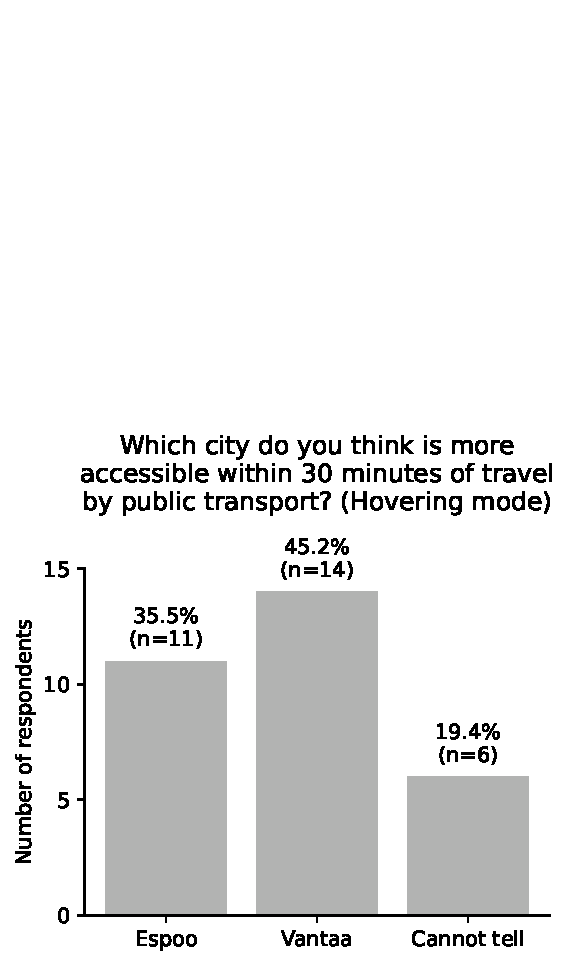
\includegraphics[width=\textwidth]{visual/figures/survey/3.pdf}
		\caption{Question 4}
		\label{fig:q 4}
	\end{subfigure}%
	\hfill
	\begin{subfigure}[b]{0.5\textwidth}
		\centering
		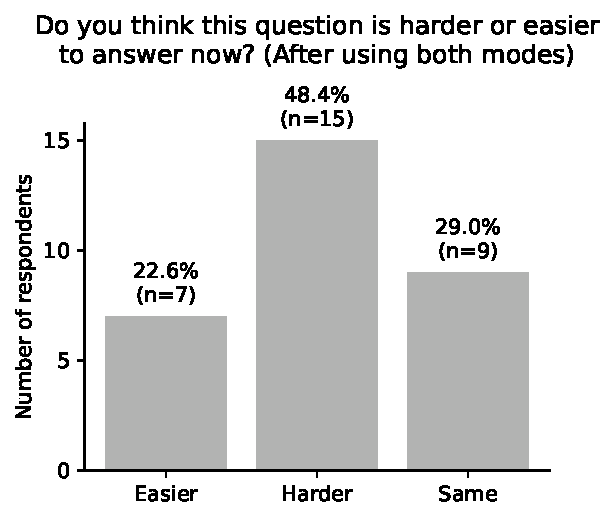
\includegraphics[width=\textwidth]{visual/figures/survey/4.pdf}
		\caption{Question 5}
		\label{fig:q 5}
	\end{subfigure}%
	\caption{Questions 4 and 5}
	\label{fig:q 4 and 5}
\end{figure}

\begin{figure}[H]
	\centering
	\begin{subfigure}[b]{0.5\textwidth}
		\centering
		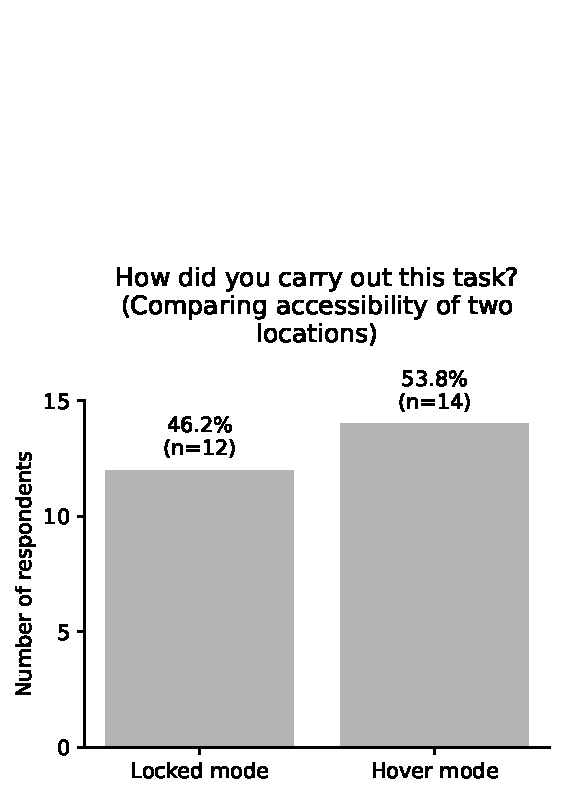
\includegraphics[width=\textwidth]{visual/figures/survey/5.pdf}
		\caption{Question 6}
		\label{fig:q 6}
	\end{subfigure}%
	\hfill
	\begin{subfigure}[b]{0.5\textwidth}
		\centering
		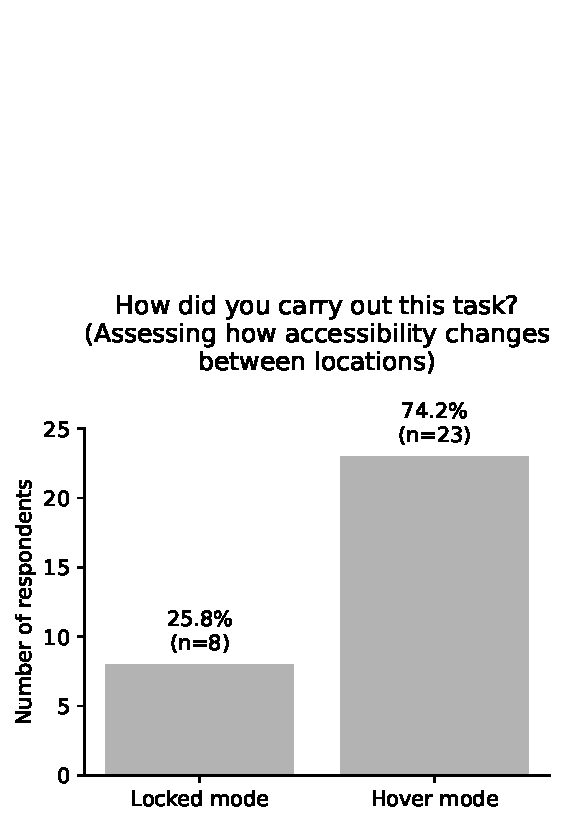
\includegraphics[width=\textwidth]{visual/figures/survey/6.pdf}
		\caption{Question 7}
		\label{fig:q 7}
	\end{subfigure}%
	\caption{Questions 6 and 7}
	\label{fig:q 6 and 7}
\end{figure}

\begin{figure}[H]
	\centering
	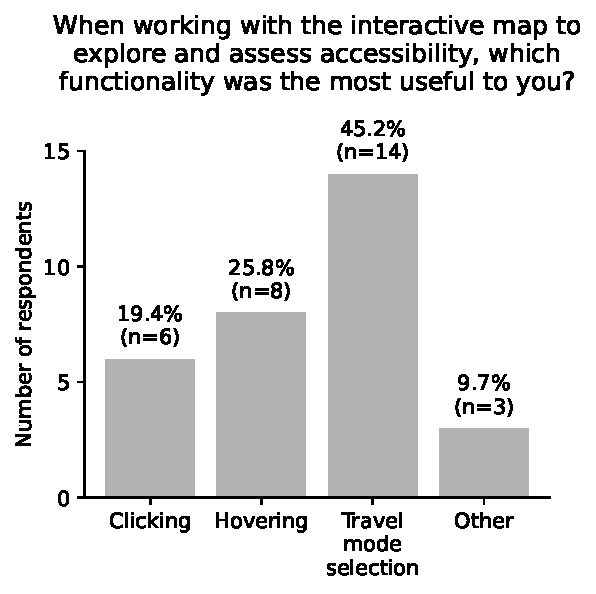
\includegraphics[width=0.5\textwidth]{visual/figures/survey/7.pdf}
	\caption{Question}
	\label{fig:q 8}
\end{figure}

\begin{figure}[H]
	\centering
	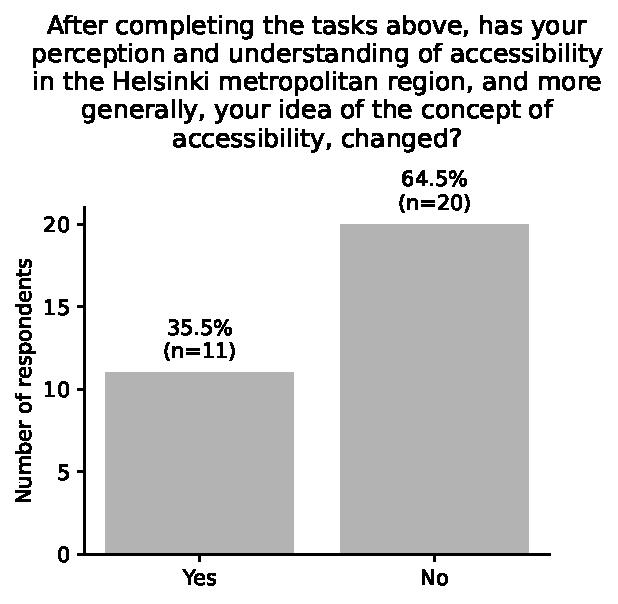
\includegraphics[width=0.5\textwidth]{visual/figures/survey/8.pdf}
	\caption{Question}
	\label{fig:q 9}
\end{figure}

\begin{figure}[H]
	\centering
	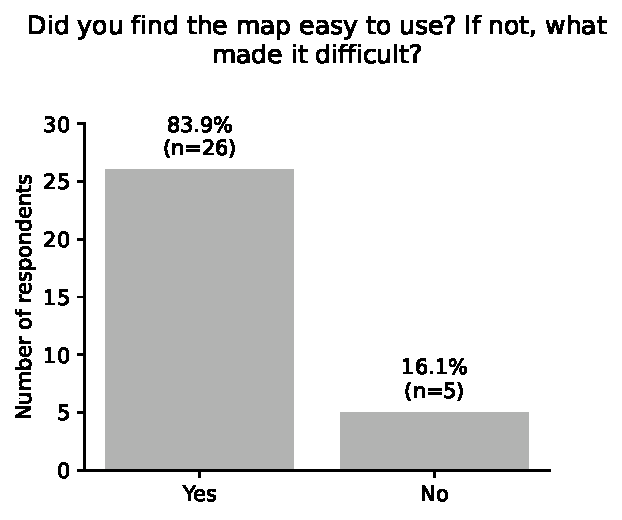
\includegraphics[width=0.5\textwidth]{visual/figures/survey/9.pdf}
	\caption{Question}
	\label{fig:q 10}
\end{figure}

\begin{figure}[H]
	\centering
	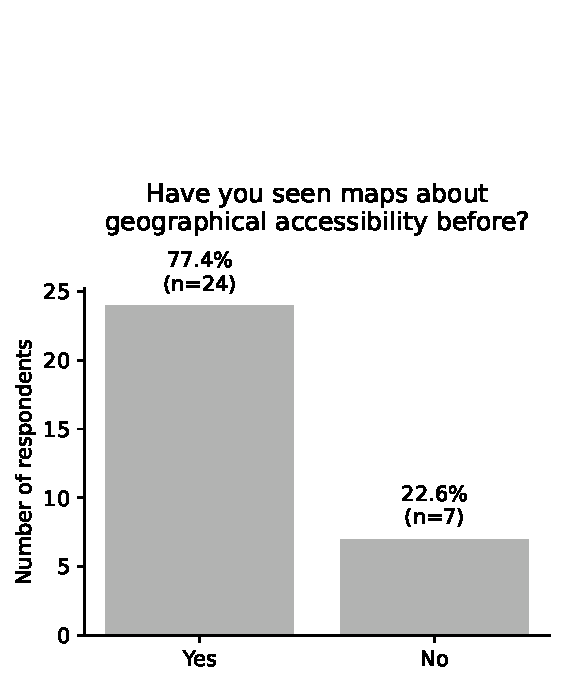
\includegraphics[width=0.5\textwidth]{visual/figures/survey/10.pdf}
	\caption{Question}
	\label{fig:q 11}
\end{figure}

\begin{figure}[H]
	\centering
	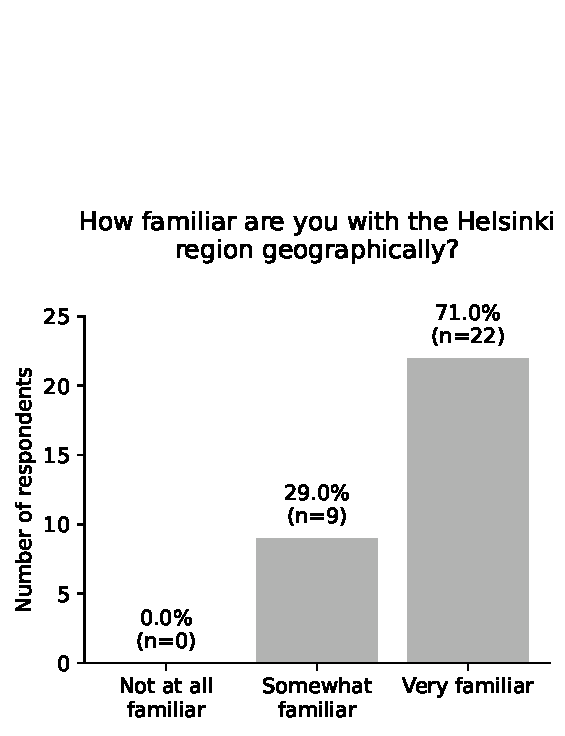
\includegraphics[width=0.5\textwidth]{visual/figures/survey/11.pdf}
	\caption{Question}
	\label{fig:q 12}
\end{figure}

\begin{figure}[H]
	\centering
	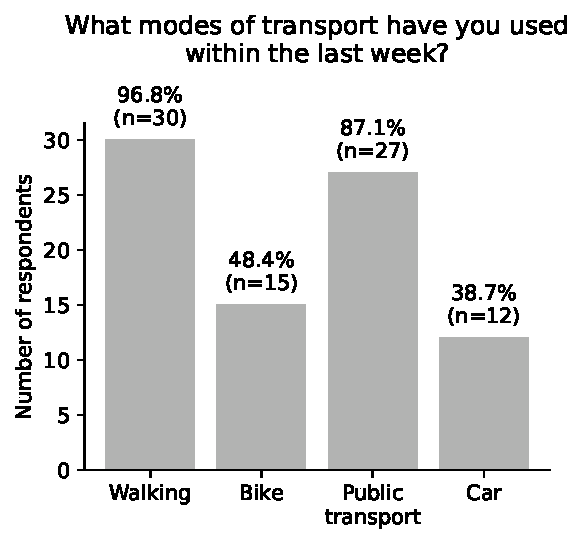
\includegraphics[width=0.5\textwidth]{visual/figures/survey/modes.pdf}
	\caption{Question}
	\label{fig:q 13}
\end{figure}

\begin{figure}[H]
	\centering
	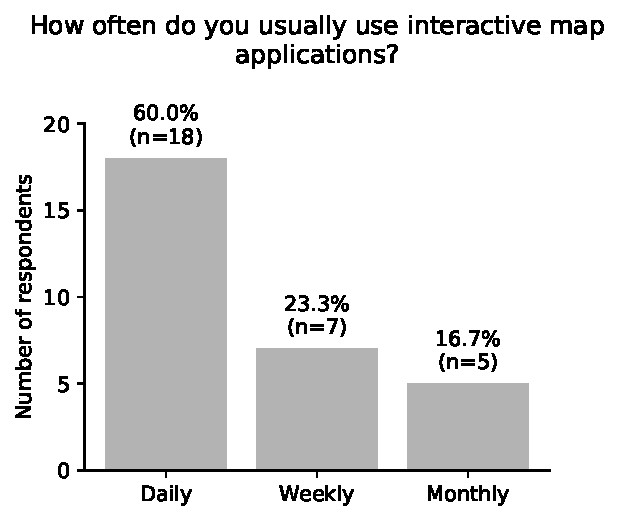
\includegraphics[width=0.5\textwidth]{visual/figures/survey/12.pdf}
	\caption{Question}
	\label{fig:q 14}
\end{figure}

\begin{figure}[H]
	\centering
	\begin{subfigure}[b]{0.5\textwidth}
		\centering
		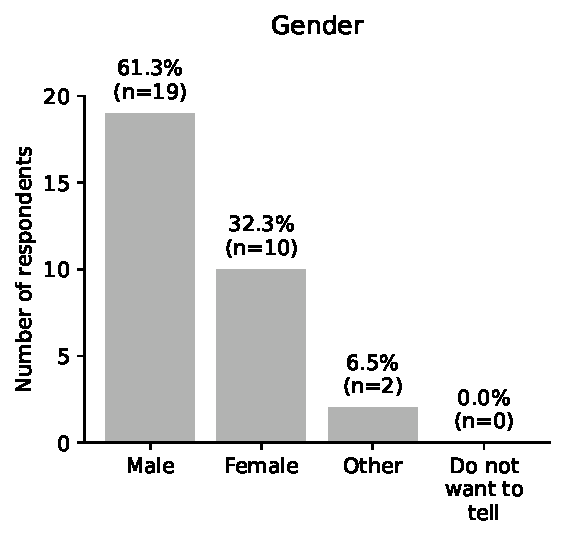
\includegraphics[width=\textwidth]{visual/figures/survey/13.pdf}
		\caption{Question 15}
		\label{fig:q 15}
	\end{subfigure}%
	\hfill
	\begin{subfigure}[b]{0.5\textwidth}
		\centering
		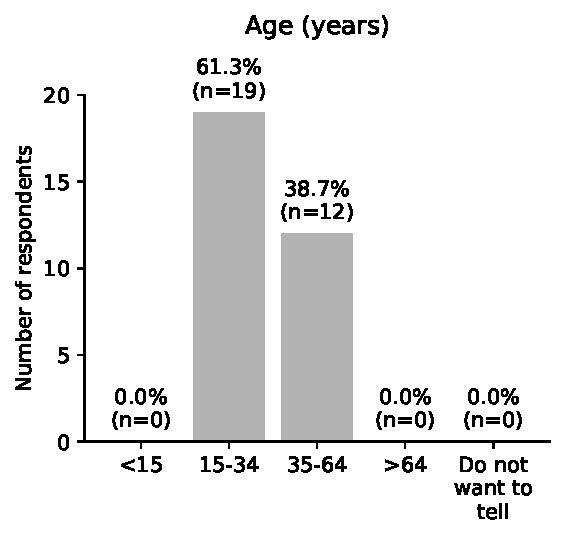
\includegraphics[width=\textwidth]{visual/figures/survey/14.pdf}
		\caption{Question 16}
		\label{fig:q 16}
	\end{subfigure}%
	\caption{Questions 15 and 16}
	\label{fig:q 15 and 16}
\end{figure}
